\renewcommand{\thefigure}{\theenumi}
\renewcommand{\thetable}{\theenumi}
%%
%\begin{enumerate}[label=\thesection.\arabic*
%,ref=\thesection.\theenumi]

\subsection{Bernoulli to Gaussian}
\begin{enumerate}[label=\thesubsection.\arabic*
,ref=\thesection.\theenumi]


\item {\em Mean :}  The mean of the bernoulli distribution is 
\begin{align}
\mu = E\brak{X_i}  = \sum_{k=0}^{1}kp_{X_i}(k) = p = \frac{1}{6}
\end{align}
\item {\em Moment:}  The moment of the distribution is defined as
\begin{align}
E\brak{X_i^r}  = \sum_{k=0}^{1}k^rp_{X_i}(k) = p = \frac{1}{6}
\end{align}

%The second moment of the bernoulli distribution is 
%\begin{align}
%E\brak{X_i}  = \sum_{k=0}^{1}kp_{X_i}(k) = p = \frac{1}{6}
%\end{align}
\item {\em Variance :}  The variance of the bernoulli distribution is defined as
\begin{align}
\sigma^2 &= E\brak{X-E\brak{X}}^2  = E\brak{X^2}-E^2\brak{X} 
\\
&=p-p^2 = p\brak{1-p} = \frac{5}{36}
\end{align}
%
The standard deviation 
\begin{align}
\sigma =  \sqrt{p\brak{1-p}}
\end{align}
%
\item {\em The Gaussian Distribution: }  Define
\begin{align}
\label{eq:bern_gauss}
G = \frac{1}{\sqrt{n}}\sum_{k=1}^{n}\frac{X_i-\mu}{\sigma}
\end{align}
%
\item {\em Approximating Binomial Using Gaussian: } From \eqref{eq:bern_gauss}
and \eqref{eq:bern_binom},
%
\begin{align}
X & \approx \sigma\sqrt{n}G + n\mu 
\\
\implies F_X(k) &= \pr{\sigma\sqrt{n}G + n\mu  \le k }
\\
 &= F_G\brak{\frac{k-n\mu}{\sigma\sqrt{n}}} \approx \phi\brak{\frac{k-n\mu}{\sigma\sqrt{n}}} 
\label{eq:bern_gaussian_cdf}
\end{align}
where 
\begin{align}
\phi_{X}(x) = \int^{x}_{-\infty} \frac{1}{\sqrt{2\pi}}e^{-\frac{x^2}{2}}, -\infty < x < \infty
\end{align}
\item The 
probability density function (PDF) 
of $G$ is
%
\begin{align}
p_{G}(x) &= \frac{d}{dx}F_{X}(x)
\\
 &=  \frac{1}{{\sigma\sqrt{n}}}\phi^{\prime}\brak{\frac{k-n\mu}{\sigma\sqrt{n}}} 
\label{eq:bern_gaussian_pdf}
\end{align}
%
For large $n$, $G$ is a continuous distribution with probability density function (PDF)
\begin{align}
p_G(x) =  \frac{1}{\sqrt{2\pi}}\exp\brak{-\frac{x^2}{2}}, -\infty < x < \infty,
\end{align}
%
\item {\em Evaluationg the Probability: }  From \ref{eq:bern_gaussian_cdf}
and \ref{eq:bern_gaussian_pdf},
\begin{align}
\pr{X \le 1 } &= F_{G}(1) = p_G(0)+p_G(1) 
\\
&\approx 
0.41299463887797094
\label{eq:bern_gauss_ans}
\end{align}
which is close to \eqref{eq:bern_binom_ans}.
%
\end{enumerate}
\subsection{Uniform to Gaussian}
\begin{enumerate}[label=\thesubsection.\arabic*
,ref=\thesection.\theenumi]

\item
Generate $10^6$ samples of the random variable
%
\begin{equation}
X = \sum_{i=1}^{12}U_i -6
\end{equation}
%
using a C program, where $U_i, i = 1,2,\dots, 12$ are  a set of independent uniform random variables between 0 and 1
and save in a file called gau.dat
\\
\solution Download the following files and execute the  C program.
\begin{lstlisting}
codes/cdf/exrand.c
codes/cdf/coeffs.h
\end{lstlisting}

%
\item
Load gau.dat in python and plot the empirical CDF of $X$ using the samples in gau.dat. What properties does a CDF have?
\\
\solution The CDF of $X$ is plotted in Fig. \ref{fig:gauss_cdf}
\begin{figure}
\centering
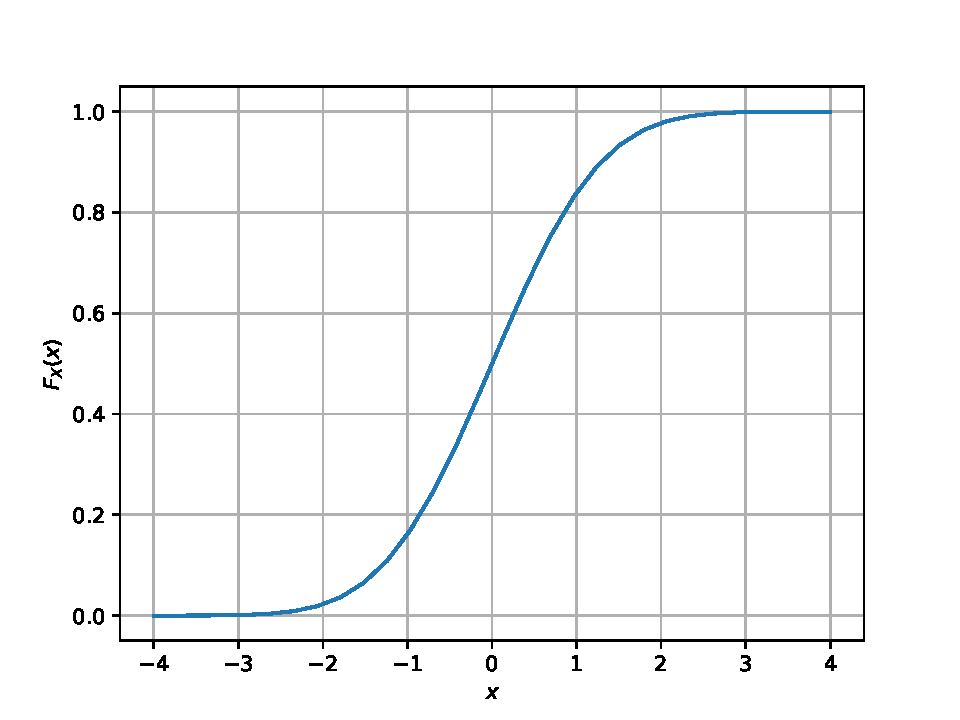
\includegraphics[width=\columnwidth]{./figs/clt/gauss_cdf}
\caption{The CDF of $X$}
\label{fig:gauss_cdf}
\end{figure}


\item
Load gau.dat in python and plot the empirical PDF of $X$ using the samples in gau.dat. The PDF of $X$ is defined as
\begin{align}
p_{X}(x) = \frac{d}{dx}F_{X}(x)
\end{align}
What properties does the PDF have?
\\
\solution The PDF of $X$ is plotted in Fig. \ref{fig:gauss_pdf} using the code below
\begin{lstlisting}
codes/clt/pdf_plot.py
\end{lstlisting}

\begin{figure}
\centering
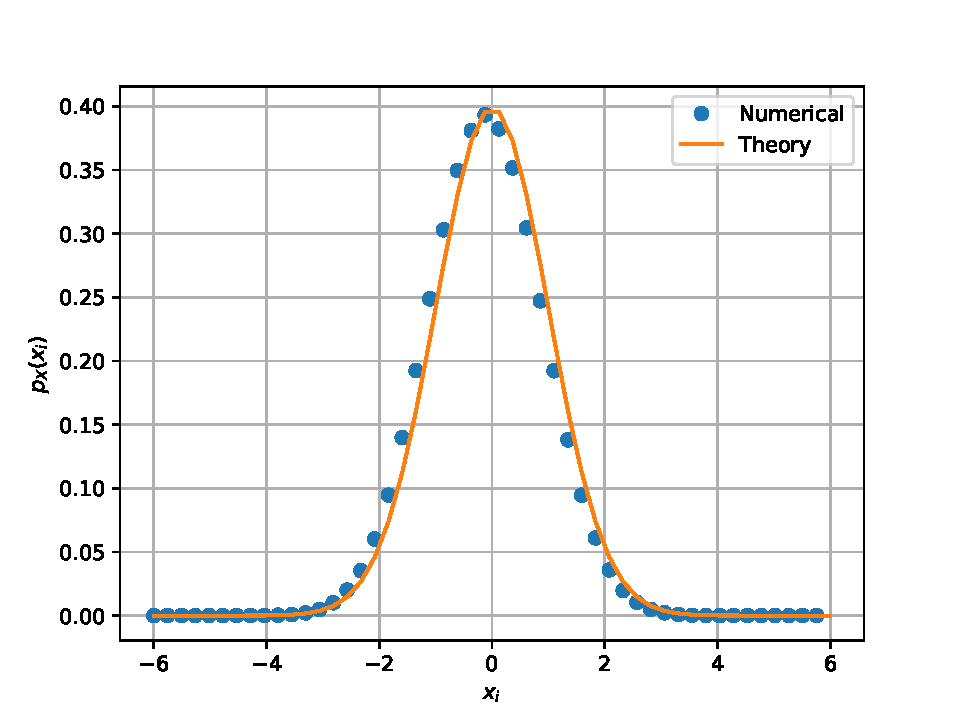
\includegraphics[width=\columnwidth]{./figs/clt/gauss_pdf}
\caption{The PDF of $X$}
\label{fig:gauss_pdf}
\end{figure}

\item Find the mean and variance of $X$ by writing a C program.
\\
\solution  Execute
\begin{lstlisting}
codes/clt/gaussian_numbers.c
\end{lstlisting}
\item Given that 
\begin{align}
p_{X}(x) = \frac{1}{\sqrt{2\pi}}\exp\brak{-\frac{x^2}{2}}, -\infty < x < \infty,
\label{eq:probman_gauss_pdf}
\end{align}
repeat the above exercise theoretically.
%
\\
\solution
Consider orthogonal vectors $\vec{m_1}$ and $\vec{m_2}$ to the given normal vector $\vec{n}$. Let, $\vec{m}$ = $\myvec{a\\b\\c}$, then
\begin{align}
\vec{m^T}\vec{n} &= 0\\
\implies\myvec{a&b&c}\myvec{3\\2\\-6} &= 0\\
\implies3a+2b-6c &= 0
\end{align}
Let a=1 and b=0 we get,
\begin{align}
\vec{m_1} &= \myvec{1\\0\\\frac{1}{2}} \label{eq:solutions/4/45/1/eq:eq1}
\end{align}
Let a=0 and b=1 we get,
\begin{align}
\vec{m_2} &= \myvec{0\\1\\\frac{1}{3}} \label{eq:solutions/4/45/1/eq:eq2}
\end{align}
Solving the equation,
\begin{align}
\vec{M}\vec{x} &= \vec{b}\label{eq:solutions/4/45/1/eq:eq3}
\end{align}
Substituting \eqref{eq:solutions/4/45/1/eq:eq1} and \eqref{eq:solutions/4/45/1/eq:eq2} in \eqref{eq:solutions/4/45/1/eq:eq3},
\begin{align}
    \myvec{1&0\\0&1\\\frac{1}{2}&\frac{1}{3}}\vec{x} &= \myvec{-3\\2\\1}\label{eq:solutions/4/45/1/eq:eq4}
\end{align}
Solving \eqref{eq:solutions/4/45/1/eq:eq4} using Singular Value Decomposition on $\vec{M}$ as follows,
\begin{align}
\vec{M}=\vec{U}\vec{\Sigma}\vec{V}^T\label{eq:solutions/4/45/1/eq:eq5}
\end{align}
Where the columns of $\vec{V}$ are the eigen vectors of $\vec{M}^T\vec{M}$ ,the columns of $\vec{U}$ are the eigen vectors of $\vec{M}\vec{M}^T$ and $\vec{S}$ is diagonal matrix of singular value of eigenvalues of $\vec{M}^T\vec{M}$. We have,
\begin{align}
\vec{M}^T\vec{M}=\myvec{\frac{5}{4}&\frac{1}{6}\\\frac{1}{6}&\frac{10}{9}}\label{eq:solutions/4/45/1/eq:eq6}\\
\vec{M}\vec{M}^T=\myvec{1&0&\frac{1}{2}\\0&1&\frac{1}{3}\\\frac{1}{2}&\frac{1}{3}&\frac{13}{36}}
\end{align}
Substituting \eqref{eq:solutions/4/45/1/eq:eq5} in \eqref{eq:solutions/4/45/1/eq:eq3},
\begin{align}
\vec{U}\vec{\Sigma}\vec{V}^T\vec{x} & = \vec{b}\\
\implies\vec{x} &= \vec{V}\vec{\Sigma^{-1}}\vec{U^T}\vec{b}\label{eq:solutions/4/45/1/eq:eq7}
\end{align}
Where $\vec{\Sigma^{-1}}$ is Moore-Penrose Pseudo-Inverse of $\vec{\Sigma}$ and is obtained by inversing only non-zero elements in $\vec{\Sigma}$\\
Calculating eigen values of $\vec{M}\vec{M}^T$,
\begin{align}
\mydet{\vec{M}\vec{M}^T - \lambda\vec{I}} &= 0\\
\implies\mydet{1-\lambda&0&\frac{1}{2}\\0&1-\lambda&\frac{1}{3}\\\frac{1}{2}&\frac{1}{3}&\frac{13}{36}-\lambda} &=0\\
\implies \lambda^3-\frac{85}{36}\lambda^2+\frac{49}{36}\lambda&=0 \label{eq:solutions/4/45/1/eq:eq8}
\end{align}
From the characteristic equation \eqref{eq:solutions/4/45/1/eq:eq8}, the eigen values of $\vec{M}\vec{M}^T$ are,
\begin{align}
\lambda_1 = \frac{49}{36} \quad
\lambda_2 = 1 \quad
\lambda_3 = 0
\end{align}
The eigen vectors of $\vec{M}\vec{M}^T$ are,
\begin{align}
\vec{u_1}=\myvec{\frac{18}{13}\\\frac{12}{13}\\1}\quad
\vec{u_2}=\myvec{\frac{-2}{3}\\1\\0}\quad
\vec{u_3}=\myvec{\frac{-1}{2}\\\frac{-1}{3}\\1}\label{eq:solutions/4/45/1/eq:eq9}
\end{align}
Normalizing the eigen vectors in equation \eqref{eq:solutions/4/45/1/eq:eq9}
\begin{align}
\vec{u_1}=\myvec{\frac{18}{7\sqrt{13}}\\\frac{12}{7\sqrt{13}}\\\frac{\sqrt{13}}{7}}\quad
\vec{u_2}=\myvec{\frac{-2}{\sqrt{13}}\\\frac{3}{\sqrt{13}}\\0}\quad
\vec{u_3}=\myvec{\frac{-7}{12}\\\frac{-7}{18}\\\frac{7}{6}}
\end{align}
Hence we obtain $\vec{U}$ as follows,
\begin{align}
\vec{U}=\myvec{\frac{18}{7\sqrt{13}}&\frac{-2}{\sqrt{13}}&\frac{-7}{12}\\\frac{12}{7\sqrt{13}}&\frac{3}{\sqrt{13}}&\frac{-7}{18}\\\frac{\sqrt{13}}{7}&0&\frac{7}{6}}\label{eq:solutions/4/45/1/eq:eq10}
\end{align}
By computing the singular values from eigen values $\lambda_1, \lambda_2, \lambda_3$ we get $\vec{\Sigma}$ as,
\begin{align}
\vec{\Sigma}=\myvec{\frac{49}{36}&0\\0&1\\0&0}
\end{align}
Calculating eigen values of $\vec{M}^T\vec{M}$,
\begin{align}
\mydet{\vec{M}^T\vec{M} - \lambda\vec{I}} &= 0\\
\implies\mydet{\frac{5}{4}-\lambda&\frac{1}{6}\\\frac{1}{6}&\frac{10}{9}-\lambda} &=0\\
\implies\lambda^2-\frac{85}{36}\lambda+\frac{49}{36} &=0
\end{align}
From the characteristic equation, the eigen values of $\vec{M}^T\vec{M}$ are,
\begin{align}
\lambda_1 = \frac{49}{36}\quad
\lambda_2 = 1
\end{align}
Hence the eigen vectors of $\vec{M}^T\vec{M}$ are,
\begin{align}
\vec{v}_1=\myvec{\frac{3}{2}\\1} \quad
\vec{v}_2=\myvec{\frac{-2}{3}\\1}
\end{align}
Normalizing the eigen vectors,
\begin{align}
\vec{v}_1=\myvec{\frac{3}{\sqrt{13}}\\\frac{2}{\sqrt{13}}} \quad
\vec{v}_2=\myvec{\frac{-2}{\sqrt{13}}\\\frac{3}{\sqrt{13}}}
\end{align}
Hence we obtain $\vec{V}$ as,
\begin{align}
\vec{V}=\myvec{\frac{3}{\sqrt{13}}&\frac{-2}{\sqrt{13}}\\\frac{2}{\sqrt{13}}&\frac{3}{\sqrt{13}}}
\end{align}
From \eqref{eq:solutions/4/45/1/eq:eq3}, the Singular Value Decomposition of $\vec{M}$ is as follows,
\begin{align}
\vec{M} = \myvec{\frac{18}{7\sqrt{13}}&\frac{-2}{\sqrt{13}}&\frac{-7}{12}\\\frac{12}{7\sqrt{13}}&\frac{3}{\sqrt{13}}&\frac{-7}{18}\\\frac{\sqrt{13}}{7}&0&\frac{7}{6}}\myvec{\frac{49}{36}&0\\0&1\\0&0}\myvec{\frac{3}{\sqrt{13}}&\frac{-2}{\sqrt{13}}\\\frac{2}{\sqrt{13}}&\frac{3}{\sqrt{13}}}^T
\end{align}
And, the Moore-Penrose Pseudo inverse of $\vec{\Sigma}$ is given by,
\begin{align}
\vec{\Sigma^{-1}} = \myvec{\frac{6}{7}&0&0\\0&1&0}
\end{align}
From \eqref{eq:solutions/4/45/1/eq:eq7} we get,
\begin{align}
\vec{U}^T\vec{b}&=\myvec{\frac{-17}{7\sqrt{13}}\\\frac{12}{\sqrt{13}}\\\frac{77}{36}}\\
\vec{\Sigma^{-1}}\vec{U}^T\vec{b}&=\myvec{\frac{-102}{49\sqrt{13}}\\\frac{12}{\sqrt{13}}}\\
\vec{x} &= \vec{V}\vec{\Sigma^{-1}}\vec{U}^T\vec{b} &= \myvec{\frac{-114}{49}\\\frac{120}{49}}\label{eq:solutions/4/45/1/eq:eq11}
\end{align}
Now we verify the solution \eqref{eq:solutions/4/45/1/eq:eq11} using,
\begin{align}
\vec{M}\vec{x}=\vec{b}
\implies\vec{M}^T\vec{M}\vec{x} = \vec{M}^T\vec{b}\label{eq:solutions/4/45/1/eqVerify}
\end{align}
On evaluating the R.H.S in \eqref{eq:solutions/4/45/1/eqVerify} we get,
\begin{align}
\vec{M}^T\vec{M}\vec{x} &= \myvec{\frac{-5}{2}\\\frac{7}{3}}\\
\implies\myvec{\frac{5}{4}&\frac{1}{6}\\\frac{1}{6}&\frac{10}{9}}\vec{x} &= \myvec{\frac{-5}{2}\\\frac{7}{3}}\label{eq:solutions/4/45/1/eq:eq12}
\end{align}
On solving the augmented matrix of \eqref{eq:solutions/4/45/1/eq:eq12} we get,
\begin{align}
\myvec{\frac{5}{4}&\frac{1}{6}&\frac{-5}{2}\\\frac{1}{6}&\frac{10}{9}&\frac{7}{3}} &\xleftrightarrow{R_1=\frac{4R_1}{5}}\myvec{1&\frac{2}{15}&-2\\\frac{1}{6}&\frac{10}{9}&\frac{7}{3}}\\
&\xleftrightarrow{R_2=R_2-\frac{R_1}{6}}\myvec{1&\frac{2}{15}&-2\\0&\frac{49}{45}&\frac{8}{3}}\\
&\xleftrightarrow{R_2=\frac{45}{49}R_2}\myvec{1&\frac{2}{15}&-2\\0&1&\frac{120}{49}}\\
&\xleftrightarrow{R_1=R_1-\frac{2R_2}{15}}\myvec{1&0&\frac{-114}{49}\\0&1&\frac{120}{49}}\label{eq:solutions/4/45/1/eq:eq13}
\end{align}
From equation \eqref{eq:solutions/4/45/1/eq:eq13}, solution is given by,
\begin{align}
\vec{x}=\myvec{\frac{-114}{49}\\\frac{120}{49}}\label{eq:solutions/4/45/1/eq:eq14}
\end{align}
From the equations \eqref{eq:solutions/4/45/1/eq:eq11} and \eqref{eq:solutions/4/45/1/eq:eq14}, the solution $\vec{x}$ is verified.

\item Let $U$ be a uniform random variable between 0 and 1.
%\begin{enumerate}[label=\thesection.\arabic*
%,ref=\thesection.\theenumi]

%
\item
Load the uni.dat file into python and plot the empirical CDF of $U$ using the samples in uni.dat. The CDF is defined as
\begin{align}
F_{U}(x) = \pr{U \le x}
\end{align}
\\
\solution  The following code plots Fig. \ref{fig:uni_cdf}
\begin{lstlisting}
codes/cdf/cdf_plot.py
\end{lstlisting}
\begin{figure}
\centering
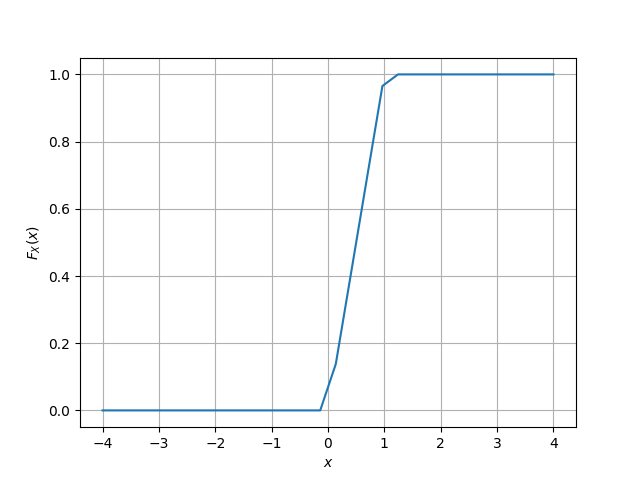
\includegraphics[width=\columnwidth]{./figs/cdf/uni_cdf}
\caption{The CDF of $U$}
\label{fig:uni_cdf}
\end{figure}

%\item Generate $10^6$ samples of $U$ using a C program and save into a file called uni.dat .
%\\


%
\item
Find a  theoretical expression for $F_{U}(x)$.

\item
The mean of $U$ is defined as
%
\begin{equation}
E\sbrak{U} = \frac{1}{N}\sum_{i=1}^{N}U_i
\end{equation}
%
and its variance as
%
\begin{equation}
\text{var}\sbrak{U} = E\sbrak{U- E\sbrak{U}}^2 
\end{equation}

Write a C program to  find the mean and variance of $U$. 
\item Verify your result theoretically given that
%
\begin{equation}
E\sbrak{U^k} = \int_{-\infty}^{\infty}x^kdF_{U}(x)
\end{equation}

\end{enumerate}



